\section{Introduction} \label{sec:introduction}

Agent-Based Model Simulation (ABMS) can address problems in basic science and applied sectors ranging from infrastructure to public health to
telecommunications.
The defining trait of agent-based modeling is cross-scale dynamics.
However, to fully realize this potential, ABMS require sufficient scale to capture the systems' emergent behaviors.

artificial life (open-ended evolution) and evolutionary epidemiology, ecology, AND blah as well as scenarios where replicating entities like cultural artifacts or computer viruses.

Emerging class of fabric-based architectures epitomized by the Cerebras Wafer Scale Engine have great promise \citep{lauterbach2021path,lie2022cerebras}.
However, needs methodological development
In particular, need to be able to observe.
Phylogenetic history is an important part of that (steal citations from arxiv papers)

\begin{figure}[htbp]
\centering
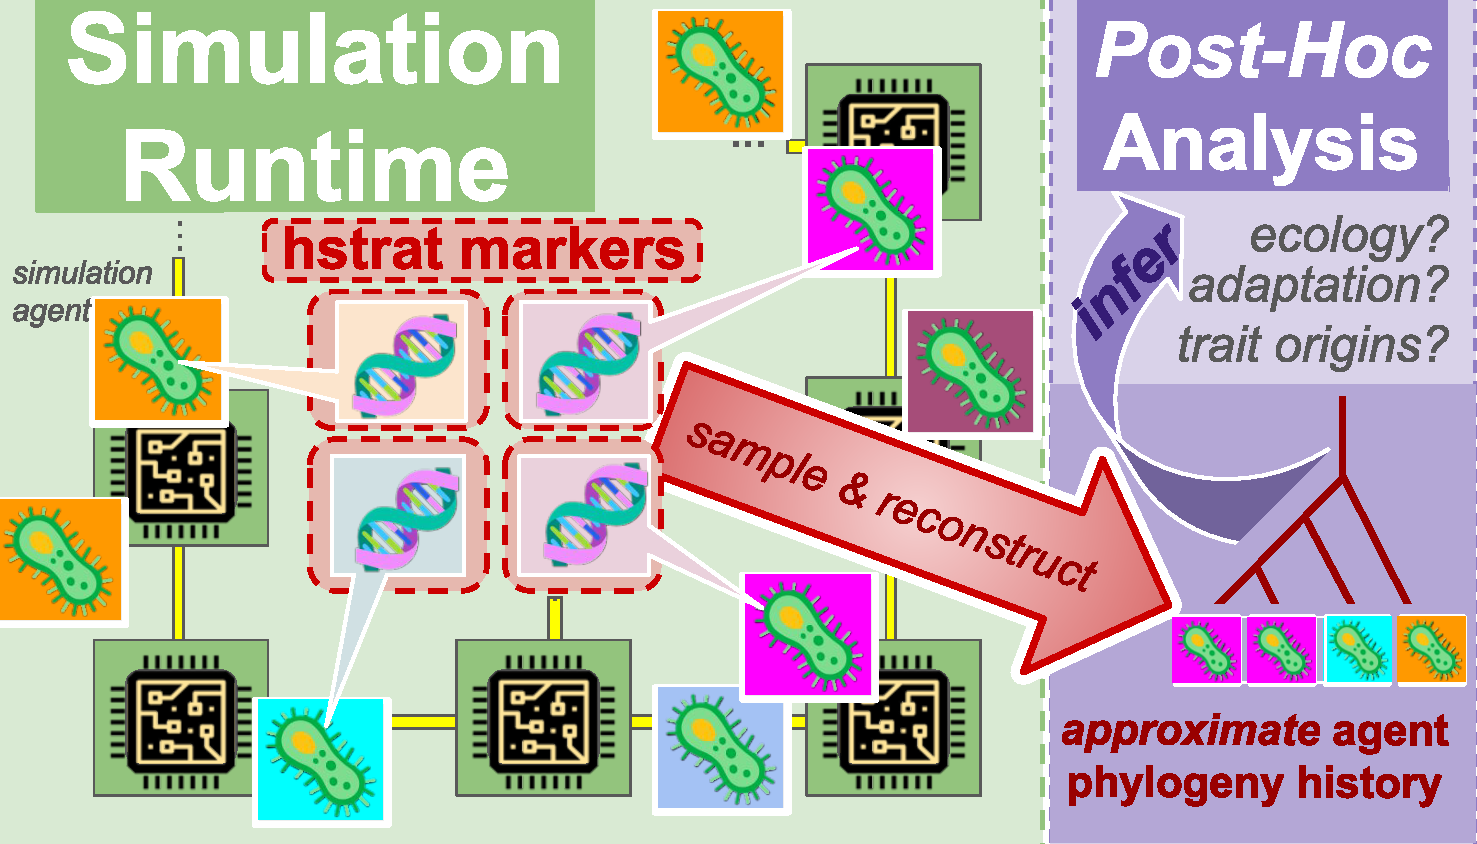
\includegraphics[width=4in]{img/runtime-posthoc-schematic.pdf}
\caption{Proposed agent-based evolutionary simulation and observation framework, using HStrat markers to estimate phylogenetic history, thereby, infer evolutionary dynamics.}
\label{fig:runtime-posthoc-schematic}
\end{figure}

A particular focus of our work is in the design of new algorithms to improve the observability of agent-based evolutionary simulations at scale through extraction of agent (e.g., pathogen) phylogenetic histories.
This information is known to provide insight into underlying evolutionary/epidemiological dynamics within a system.
Further, comparison of observed phylogenies against simulation phylogenies can be used to evaluate hypotheses for underlying dynamics within real-life evolutionary/epidemiological systems.

Historically, simulation phylogenies have typically only been collected using a centralized, complete record-keeping approach suited to serial simulation.
To overcome this limitation, we have proposed a new class of reconstruction-based approaches to phylogenetic tracking in silico.
These approaches require no data collection during simulation runtime; instead, they use post hoc comparisons between end-state agents to deduce approximate phylogenetic history.

\section{Objectives} \label{sec:objectives}

Technical demonstration and evaluation of methodology stitched together into answering technical questions about huge-scale phylogenetic structure that existing approaches have yet been able to address.

Objective one: technology demonstration of reconstruction at wafer scale.
Validate by running under two simple evolutionary conditions that expect to produce different phylogenetic structure.
See if we can recover that phylogenetic structure.

Also, observe scalability of asynchronous evolutionary approach.

Objective two: are phylogenetic structure metrics scale invariant?
Run several evolutionary conditions with small colletions of PEs and large collections of PEs
Test for differences in phylogenetic structure metrics.
(how to control for reconstruction quality?)

Objective three: what is the relationship between individual phylogenies and species-level phylogenies?

Another objective: does streaming samples off the chip asynchronously bias phylometrics (as opposed to collecting everything all at the end.

Relatedly: are phylometrics time invariant to duration of simulation?


Early evaluations of this revised approach have achieved high-quality reconstruction of phylogenetic histories for tens of thousands of fully-distributed agents using just 96 bits of tracking information per agent.


Order-of-magnitude increases in tractable model scales are possible through 1) Parallel Discrete Event Simulation (PDES) approaches and 2) emerging high-performance computing (HPC) accelerator hardware.
These approaches potentially synergize; in the emerging class of fabric-based architectures, compute elements interface primarily with neighbors, a paradigm suited to the locally-structured interaction networks common in ABMS/PDES.
Of course, these approaches also pose unique challenges, many centering on difficulty maintaining sufficient historical state to run the model and collect data without exceeding the tight memory limits of processor elements.
%In particular, the limited communication with external (``host'') devices in fabric-based accelerator architectures inhibits retrieving data from ABMS/PDES.
%but these approaches pose challenges individually and in combination.
% Success hinges on reconciling the irregular computational profile of PDES with the capabilities (and limitations) of accelerator hardware.
%One major performance challenge is limitations to host-device communication.
%Notably, in the emerging class of fabric-based architectures, many accelerator compute elements interface only with local neighbors rather than with an overarching host, creating communication challenges.

To advance on this front, we propose a fundamental re-frame of simulation that shifts from a paradigm of ``complete,'' deterministic data observability to dynamic, inquiry-driven sampling akin to approaches traditionally used to study physical systems.
In exchange, this relaxation to ``best-effort'' observability addresses bandwidth/storage limitations, enables on-the-fly queries, and tolerates intermittent disruption.
We will leverage the space-time memory paradigm to provide an efficient, robust interface between PDES and dynamic, inquiry-driven data extraction while preserving the integrity of underlying simulation.


example \citep{gagliardi2019international}


We are interested in developing applications of the Cerebras CS-2 to agent-based evolutionary modeling of epidemiological scenarios.
The unique capabilities of the CS-2 platform will allow us to push the boundaries of model-based inquiry, allowing investigation of new questions at the magnitude of continental or global-scale population structure and at the resolution of individual-level immunological responses.

A particular focus of our work is in the design of new algorithms to improve the observability of agent-based evolutionary simulations at scale through extraction of agent (e.g., pathogen) phylogenetic histories.
This information is known to provide insight into underlying evolutionary/epidemiological dynamics within a system.
Further, comparison of observed phylogenies against simulation phylogenies can be used to evaluate hypotheses for underlying dynamics within real-life evolutionary/epidemiological systems.

Historically, simulation phylogenies have typically only been collected using a centralized, complete record-keeping approach suited to serial simulation.
To overcome this limitation, we have proposed a new class of reconstruction-based approaches to phylogenetic tracking in silico.
These approaches require no data collection during simulation runtime; instead, they use post hoc comparisons between end-state agents to deduce approximate phylogenetic history.


With access to CS-2 hardware, we plan to evaluate the viability of reconstruction-based methodology for in silico phylogenetic tracking at scale in production and then incorporate it within large-scale epidemiological modeling experiments performed via a custom CSL kernel.

I am collaborating on this project with Dr. Emily Dolson (Michigan State University), Dr. Luis Zaman (University of Michigan), and undergraduate researchers Anika Ranjan and Connor Yang, cc'ed.



\noindent\textbf{Introduction:}
Agent-Based Model Simulation (ABMS) can address problems in sectors ranging from infrastructure to public health to
telecommunications.
However, to fully realize this potential, ABMS require sufficient scale to capture the systems' emergent behaviors.
Order-of-magnitude increases in tractable model scales are possible through 1) Parallel Discrete Event Simulation (PDES) approaches and 2) emerging high-performance computing (HPC) accelerator hardware.
These approaches potentially synergize; in the emerging class of fabric-based architectures, compute elements interface primarily with neighbors, a paradigm suited to the locally-structured interaction networks common in ABMS/PDES.
Of course, these approaches also pose unique challenges, many centering on difficulty maintaining sufficient historical state to run the model and collect data without exceeding the tight memory limits of processor elements.
%In particular, the limited communication with external (``host'') devices in fabric-based accelerator architectures inhibits retrieving data from ABMS/PDES.
%but these approaches pose challenges individually and in combination.
% Success hinges on reconciling the irregular computational profile of PDES with the capabilities (and limitations) of accelerator hardware.
%One major performance challenge is limitations to host-device communication.
%Notably, in the emerging class of fabric-based architectures, many accelerator compute elements interface only with local neighbors rather than with an overarching host, creating communication challenges.

To advance on this front, we propose a fundamental re-frame of simulation that shifts from a paradigm of ``complete,'' deterministic data observability to dynamic, inquiry-driven sampling akin to approaches traditionally used to study physical systems.
In exchange, this relaxation to ``best-effort'' observability addresses bandwidth/storage limitations, enables on-the-fly queries, and tolerates intermittent disruption.
We will leverage the space-time memory paradigm to provide an efficient, robust interface between PDES and dynamic, inquiry-driven data extraction while preserving the integrity of underlying simulation.
% By also applying this paradigm to data used within the PDES, we will enable memory-efficient computation without synchronization.
%(e.g., visualization, monitoring ``what-if'' interventions),
%by bursting communication within underlying simulation.

While such an approach promises benefits across scientific domains, we are focusing on evolutionary epidemiology, which hinges on cross-scale dynamics and employs mature, widely-accepted sampling-based surveillance methods.
Traditional epidemiological models have yet to incorporate detailed pathogen evolution (and vice versa), likely due to %the
scaling challenges.% associated with representing individual pathogens in the model.
Nevertheless, pathogen evolution needs to be considered when making public health policy decisions.
To capture emergent evolutionary trade-offs, these models must implement individual pathogens as first-class agents.
%To depict evolution on a realistically complex fitness landscape, these models must represent individual pathogens as agents.%
To run massive models necessary to test our ``best effort" observability approaches, we will target the 850,000 core Cerebras Wafer Scale Engine, which features a fabric architecture epitomic of emerging accelerator memory and I/O challenges; however, our proposed methodology generalizes to other domains and HPC hardware systems.

% One common purpose for Agent-Based Model Simulations (ABMS) is to reproduce a real-world phenomenon in a digital context where the behavior of the system can be perfectly observed.
% Often, the behavior of interest relates to interactions or relationships between agents.
% The inter-agent synchronization that such data collection requires can be a major obstacle to unifying ABMS with Parallel Discrete Event Simulations (PDES).
% For example, classical approaches to tracking phylogenetic (i.e., ancestry) relationships in ABMS representing evolutionary phenomena incur a dramatic slowdown in parallel computing contexts \citep{morenoHereditaryStratigraphyGenome2022}.
% We propose a space time memory approach to scalable data collection that will enable development of unified ABMS/PDES systems.

% Specifically, our approach will center on a paradigm we term ``best-effort observability.''
% Traditional serial ABMS generally operate on the assumption of
% In contrast, we propose sacrificing a tunable amount of data/precision to increase the scale of modelling that can tractably be achieved.

\vspace{.5em}
\noindent\textbf{Prior research:}
In pilot work with dynamically curated space-time memory buffers, we have achieved highly-scalable phylogenetic tracking in ABMS modelling of evolutionary processes \citep{morenoHstratPythonPackage2022, morenoHereditaryStratigraphyGenome2022}.
Our approach, hereditary stratigraphy (HStrat), uses a reconstruction-based strategy akin to how biologists build phylogenies.
Using heritable generational fingerprints, we achieve fast, accurate reconstruction.
To prevent $\mathcal{O}(n)$ space complexity, not all fingerprints can be kept.
Instead, we use a constant-time indexing scheme to map a stream of fingerprints onto a fixed-width memory buffer such that entries evicted by new placements maintain a temporally-representative sampling over elapsed time, either evenly (``steady'') or recency-biased (``tilted'') (Fig. \ref{fig:hstrat-schematic}).
Time stamps can be positionally inferred  --- a several-fold savings for small data objects. For example, single-bit checkpoints produce good quality phylogenies using only 12 bytes per genome \citep{moreno2023toward}.
% Instead,  these fingerprints on a rolling basis required development of


% The input to this problem is a stream of data too large to be fully retained. To solve this problem, one can identify various algorithms describing policies for determining which data to retain. Previously, we have identified a range of highly-efficient policy algorithms that allow the user to precisely tune 1) the space complexity, and 2) the precision with which historical states of the data stream can be known.

% gives users control over tradeoffs between space complexity and the precision with which phylogenies can be reconstructed.

% We have demonstrated both experimentally and analytically that HStrat dramatically increases the scale (in terms of population size and number of generations) at which evolutionary ABMS producing phylogenetic data can tractably be run, particularly in parallel and distributed computing contexts.
% Additionally, we have explored the impacts of different strategies for determining which data to keep (e.g. whether and to what extent to prioritize recent data).
\vspace{.5em}
\noindent\textbf{Objectives:} Our goals for this grant are two-fold:
% \setlist{nolistsep}
\begin{enumerate}%[noitemsep]
% facilitate the development of unified ABMS/PDES by
\item To advance capabilities of highly-distributed ABMS/PDES by leveraging newly-developed space-time memory curation algorithms for buffering time series data, managing semi-persistent simulation elements, and tracking hierarchical object histories.% (e.g., copy trees).
%(e.g., fomite reservoirs or host immune memory)
\item To develop strategies for partial, best-effort observability of large-scale PDES running on fabric-style accelerators that focus limited available bandwidth and storage on specific hypotheses.
\end{enumerate}


% previous work: we're going to scale up the existing approach AND we're going to transplant this to other partial observability
% we're annotating agents with space-time memory
% interface with eachother without synchroniztation and send out
% best-effort paired garbage collection (implicit, one in one out; stream in, worst out)
% make connection of reference counting to pruning a phylogeny?

%In practice, such precision is usually unnecessary for multiple reasons: 1) data will need to be summarized  or otherwise simplified for analysis anyway, and 2) levels of precision in agent-based models so far exceed the precision of real world measurements that the extra information is  not actionable.

% \textbf{Overall approach:} Our proposed approach will build on prior work tackling what we have termed the \textit{streaming curation problem}. The input to this problem is a stream of data too large to be fully retained. To solve this problem, one can identify various algorithms describing policies for determining which data to retain. Previously, we have identified a range of highly-efficient policy algorithms that allow the user to precisely tune 1) the space complexity, and 2) the precision with which historical states of the data stream can be known.

% hook into cerebras is an accelerator

% Talk about phylogenies

% Talk about what else we're going to do
% - Run hstrat on cerebrus
% - Eye of sauron




% \input{fig/model-schematic}
\vspace{.5em}

\noindent\textbf{Application areas:} Our focus is epidemiological modeling.
We will use our expanded scale to capture within-host and between-host pathogen behaviors, and evaluate evolved pathogen traits that balance trade-offs occurring across scales.
Using space-time buffers, we will support 1) asynchronous interactions between simulation components (e.g., host agents, pathogen agents, geographic locales) and 2) dynamic, inquiry-driven data extraction (Fig. \ref{fig:model-schematic}).

% ADDITIONAL IDEAS
% collaboratorships/scientific networking
% generally, having a record of recent interactioons with other agents
% patent record/phylogeny of ideas in "scientific enterprise"
% generally, agent behavior based on a rough history of recent experience
Proposed strategies will generalize across ABMS/PDES domains where sampled observations can fulfill experimental objectives.
For example, in congestion models (e.g., road traffic, internet traffic), statistical measures of net bandwidth or backups at critical sites can suffice to assess network-level outcomes and coarsened histories attached to individual agents can show underlying dynamics (e.g., position across time).
%